\documentclass[a4paper, 10pt]{article}\usepackage[]{graphicx}\usepackage[]{xcolor}
% maxwidth is the original width if it is less than linewidth
% otherwise use linewidth (to make sure the graphics do not exceed the margin)
\makeatletter
\def\maxwidth{ %
  \ifdim\Gin@nat@width>\linewidth
    \linewidth
  \else
    \Gin@nat@width
  \fi
}
\makeatother

\definecolor{fgcolor}{rgb}{0.345, 0.345, 0.345}
\newcommand{\hlnum}[1]{\textcolor[rgb]{0.686,0.059,0.569}{#1}}%
\newcommand{\hlstr}[1]{\textcolor[rgb]{0.192,0.494,0.8}{#1}}%
\newcommand{\hlcom}[1]{\textcolor[rgb]{0.678,0.584,0.686}{\textit{#1}}}%
\newcommand{\hlopt}[1]{\textcolor[rgb]{0,0,0}{#1}}%
\newcommand{\hlstd}[1]{\textcolor[rgb]{0.345,0.345,0.345}{#1}}%
\newcommand{\hlkwa}[1]{\textcolor[rgb]{0.161,0.373,0.58}{\textbf{#1}}}%
\newcommand{\hlkwb}[1]{\textcolor[rgb]{0.69,0.353,0.396}{#1}}%
\newcommand{\hlkwc}[1]{\textcolor[rgb]{0.333,0.667,0.333}{#1}}%
\newcommand{\hlkwd}[1]{\textcolor[rgb]{0.737,0.353,0.396}{\textbf{#1}}}%
\let\hlipl\hlkwb

\usepackage{framed}
\makeatletter
\newenvironment{kframe}{%
 \def\at@end@of@kframe{}%
 \ifinner\ifhmode%
  \def\at@end@of@kframe{\end{minipage}}%
  \begin{minipage}{\columnwidth}%
 \fi\fi%
 \def\FrameCommand##1{\hskip\@totalleftmargin \hskip-\fboxsep
 \colorbox{shadecolor}{##1}\hskip-\fboxsep
     % There is no \\@totalrightmargin, so:
     \hskip-\linewidth \hskip-\@totalleftmargin \hskip\columnwidth}%
 \MakeFramed {\advance\hsize-\width
   \@totalleftmargin\z@ \linewidth\hsize
   \@setminipage}}%
 {\par\unskip\endMakeFramed%
 \at@end@of@kframe}
\makeatother

\definecolor{shadecolor}{rgb}{.97, .97, .97}
\definecolor{messagecolor}{rgb}{0, 0, 0}
\definecolor{warningcolor}{rgb}{1, 0, 1}
\definecolor{errorcolor}{rgb}{1, 0, 0}
\newenvironment{knitrout}{}{} % an empty environment to be redefined in TeX

\usepackage{alltt}
% package accents
\usepackage[utf8]{inputenc}% input en utf8
\usepackage[french]{babel}% typo française
\usepackage[T1]{fontenc}% accents out en format T1
\usepackage{csquotes}% typo française (guillemets)

% packages maths (les plus courants)
\usepackage{amsmath}
\usepackage{mathtools}
\usepackage{amsfonts}
\usepackage{amssymb}
\usepackage{mathabx}
\usepackage{cases}

\usepackage{enumerate} % listes

% biblio
\usepackage[bibstyle=verbose, citestyle=verbose-trad1, backend=biber, isbn=false, url=false, doi=false]{biblatex}
\bibliography{Biblio.bib}
\DeclareNameAlias{sortname}{family-given} % nom de famille en premier

% mise en forme des paragraphes
\usepackage{parskip}% saut de lignes en fin de paragraphe
\let\EndItemize\enditemize
\def\enditemize{\EndItemize\bigskip}% sauts de ligne en fin d'environnement itemize

% tables et figures
\usepackage{multirow} % permet de fusionner les colonnes
\usepackage{graphicx} % admet les figures
\usepackage{array} % types particuliers de tableaux
\usepackage{tabularx} % autres tableaux, notamment pour gérer les doubles traits de séparation (voir hhline)
\usepackage[hang,small]{caption} % mise en forme du caption


% mise en page
\usepackage[colorlinks=true, urlcolor=blue, linkcolor=gray, menucolor=black]{hyperref} % liens hypertextes
\usepackage[bottom]{footmisc} % mise en forme des notes de bas de page "\footnote"
\usepackage[left=2cm,right=2cm,top=2cm,bottom=2cm]{geometry} % marges
\setcounter{tocdepth}{2}

% page de garde/titre (en fonction de la classe de document)
\usepackage{titling} % pour le titre en gras
\author{\href{mailto:julioricardo.davalos@ehess.fr}{Julio Ricardo Davalos}}
\title{Petite introduction à \LaTeX{} en Sciences Sociales}
\date{Septembre 2022}

% pour tableaux stargazer et kable
\usepackage{dcolumn}
\usepackage{rotating}
\usepackage{graphicx}
\usepackage{xstring}
\usepackage{array} 
\usepackage{tabularx}
\usepackage{multirow}
\usepackage{booktabs}

% macros
\newcommand{\etoiles}{%
	\begin{center}
    $\ast$\\ $\ast$~\hspace*{2mm}~$\ast$\\
  \end{center}
}

%-------------------------------Options pour Sweave--------------------------------


\IfFileExists{upquote.sty}{\usepackage{upquote}}{}
\begin{document}

\maketitle
\tableofcontents

\section*{Section non numérotée}\addcontentsline{toc}{section}{Section non numérotée}
\subsection*{Sous-section non numérotée}
Ce document a pour but d'introduire à l'utilisation du langage \LaTeX{} à un public venant des SHS. En effet, ce langage est assez commun dans les sciences expérimentales mais reste inconnu (ou alors connu que de nom) pour beaucoup de chercheurs et étudiants en SHS. Cela peut être dû à son côté austère ou encore au fait qu'il peut paraître destiné uniquement à mettre en forme des mathématiques, capacité que l'on peut considérer comme secondaire voire superflue dans notre cas.

\section{Section numérotée}
\subsection{Sous-section numérotée}


\begin{figure}[!ht]
	\caption{Une image choisie complètement au hasard}\label{bourdieu}
	\centering
	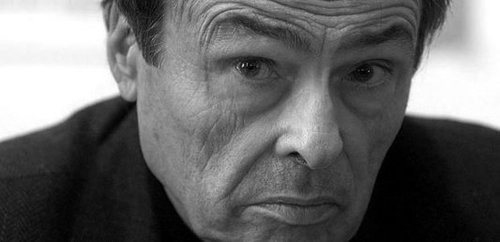
\includegraphics[scale=0.4]{Images/bourdieu.jpg}
\end{figure}
Je cite la figure \ref{bourdieu}

  \begin{table}[!ht]
    \caption{Un tableau vide et centré}
    \centering
    \begin{tabular}{|l|c|}
    \hline
    Case $(1,1)$ oudfhodfhdfvgsdf sdf & Case $(1,2)$ \\
    \hline
     Case $(2,1)$ & Case $(2,2)$ \\
    \hline
    \end{tabular}
  \end{table}
  
 \begin{figure}[!ht]
  \begin{tabular}{cc}
    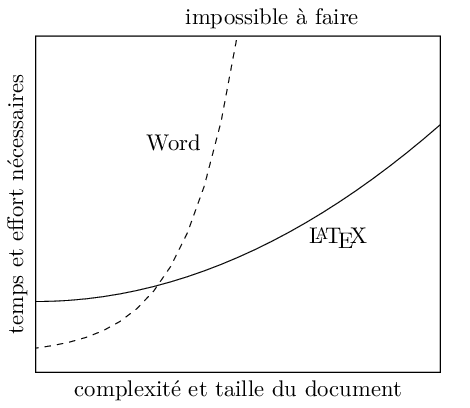
\includegraphics[width=0.5\textwidth]{Images/latex_word.png} & 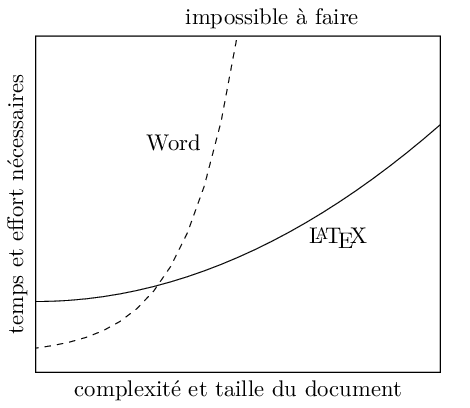
\includegraphics[width=0.5\textwidth]{Images/latex_word.png} \\
    \end{tabular}
 \end{figure}

\begin{itemize}
  \item point 1
  \item[$\Rightarrow$] point 2
\end{itemize}

\begin{enumerate}[(a)]% avec le package enumerate
  \item point 1
  \item point 2
\end{enumerate}

\textbackslash\\
\textasciitilde

\textasciicircum

\enquote{guillemets, \enquote{autres guillemets}}

\textit{italique}
\emph{italique, \emph{pas italique}}

\textbf{gras}



\cite{Rouquette2011}\footcite{Rouquette2011}
\nocite{Rouquette2011}
\nocite{*}

\section{Sweave}
\begin{knitrout}
\definecolor{shadecolor}{rgb}{0.969, 0.969, 0.969}\color{fgcolor}\begin{kframe}
\begin{verbatim}
## [1] "une commande R"
\end{verbatim}
\end{kframe}
\end{knitrout}




\begin{knitrout}
\definecolor{shadecolor}{rgb}{0.969, 0.969, 0.969}\color{fgcolor}\begin{kframe}
\begin{verbatim}
##          n    % val%
## cerise 103 10.3 10.3
## fraise 516 51.6 51.6
## mangue 191 19.1 19.1
## orange 190 19.0 19.0
\end{verbatim}
\end{kframe}
\end{knitrout}


\begin{knitrout}
\definecolor{shadecolor}{rgb}{0.969, 0.969, 0.969}\color{fgcolor}\begin{table}[!h]

\caption{\label{tab:freqchoix}Fréquence des choix}
\centering
\begin{tabular}[t]{lrrr}
\toprule
  & n & \% & val\%\\
\midrule
cerise & 103 & 10.3 & 10.3\\
fraise & 516 & 51.6 & 51.6\\
mangue & 191 & 19.1 & 19.1\\
orange & 190 & 19.0 & 19.0\\
\bottomrule
\end{tabular}
\end{table}

\end{knitrout}



% Table created by stargazer v.5.2.3 by Marek Hlavac, Social Policy Institute. E-mail: marek.hlavac at gmail.com
% Date and time: mer., sept. 07, 2022 - 17:15:46
\begin{table}[!htbp] \centering 
  \caption{Trois beaux modèles} 
  \label{} 
\begin{tabular}{@{\extracolsep{5pt}}lccc} 
\\[-1.8ex]\hline 
\hline \\[-1.8ex] 
 & \multicolumn{3}{c}{\textit{Dependent variable:}} \\ 
\cline{2-4} 
\\[-1.8ex] & choix\_fraise & choix\_cerise & nb\_fruits \\ 
\\[-1.8ex] & \textit{logistic} & \textit{logistic} & \textit{OLS} \\ 
\\[-1.8ex] & (1) & (2) & (3)\\ 
\hline \\[-1.8ex] 
 age & 0.003 & $-$0.0003 & 0.031$^{***}$ \\ 
  & (0.002) & (0.004) & (0.001) \\ 
  & & & \\ 
 aime\_kiwiOui & $-$0.059 & $-$0.231 & 0.948$^{***}$ \\ 
  & (0.161) & (0.280) & (0.085) \\ 
  & & & \\ 
 aime\_melonOui & $-$0.103 & 0.256 & 1.062$^{***}$ \\ 
  & (0.127) & (0.210) & (0.067) \\ 
  & & & \\ 
 aime\_ananasOui & $-$0.137 & 0.613$^{**}$ & 1.048$^{***}$ \\ 
  & (0.136) & (0.251) & (0.072) \\ 
  & & & \\ 
 Constant & 0.067 & $-$2.686$^{***}$ & 1.972$^{***}$ \\ 
  & (0.175) & (0.316) & (0.092) \\ 
  & & & \\ 
\hline \\[-1.8ex] 
Observations & 1,000 & 1,000 & 1,000 \\ 
R$^{2}$ &  &  & 0.557 \\ 
Adjusted R$^{2}$ &  &  & 0.555 \\ 
Log Likelihood & $-$690.594 & $-$327.360 &  \\ 
Akaike Inf. Crit. & 1,391.188 & 664.720 &  \\ 
Residual Std. Error &  &  & 1.056 (df = 995) \\ 
F Statistic &  &  & 312.946$^{***}$ (df = 4; 995) \\ 
\hline 
\hline \\[-1.8ex] 
\textit{Note:}  & \multicolumn{3}{r}{$^{*}$p$<$0.1; $^{**}$p$<$0.05; $^{***}$p$<$0.01} \\ 
\end{tabular} 
\end{table} 



\begin{knitrout}
\definecolor{shadecolor}{rgb}{0.969, 0.969, 0.969}\color{fgcolor}\begin{figure}[ht!]
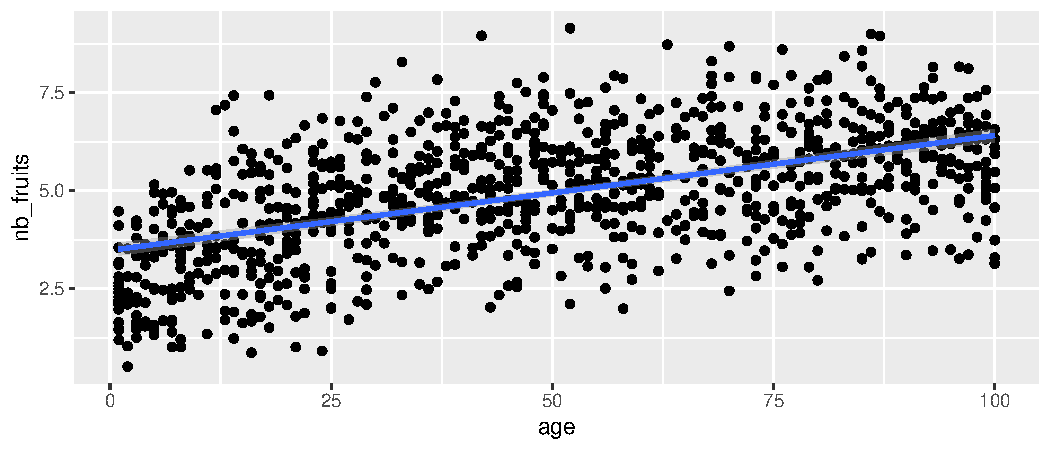
\includegraphics[width=\maxwidth]{Sorties/Graphunnamed-chunk-7-1} \caption[Nombre de fruits estimés en fonction de l'âge]{Nombre de fruits estimés en fonction de l'âge}\label{nbfruits_ageunnamed-chunk-7}
\end{figure}

\end{knitrout}

\newpage
\printbibliography
\end{document}

